\chapter{Непрерывные функции от одной переменной}

\section{Лекция \#12. Понятие непрерывного отображения на прямой}


\subsection{Отображения}
Пусть $X,Y$ -- два множества, $R(x,y)$ -- отношение между $x \in X$, $y \in Y$. \textit{График} $\Gamma(R)$ отношения $R$ определяется следующим образом
\[
 X \times Y \supseteq \Gamma(R) : = \{(x,y) \, :\, (x,y) \in R\}.
\]

Пусть $X,Y$ -- два множества, $R(x,y)$ -- отношение между $x \in X$, $y \in Y$. Говорят, что $R$ \textit{функционально по $y$}, если для \textbf{каждого} $x\in X$ существует \textbf{один и только один} такой элемент $y\in Y$, что $R(x,y)$ истинно.

График $F$ такого отношения называется \textit{функциональным графиком} в $X \times Y$. Его можно также охарактеризовать следующим образом:  для каждого $x \in X$ существует один и только один такой элемент $y \in Y$, что $(x,y) \in R$; этот элемент называется \textit{значением} $F$ в $x$ и обозначается символом $F(x)$.

\begin{definition}
 Функциональный график в $X \times Y$ называется также \textit{отображением $X$ в $Y$} или \textit{функцией, определённой в $X$ и принимающей значения в $Y.$}    
\end{definition}

Мы также будем записывать такое отображение в виде $F:X \to Y$, понимая под этим, что каждому $x \in X$ ставится в соответствие ровно один $y  = F(x)\in Y$.

\begin{mydangerr}{\bf !}
    Таким образом, мы считаем, что $F$ определено на всём $X.$ 
\end{mydangerr}
~

Мы переформулируем определение отображения в более удобном для нас виде.

\begin{definition}
    Отображением множества $X$ в множество $Y$ называется тройка $(X,Y,F)$, составленная из $X,Y$, и правила $F$, ставящего в соответствие \textbf{каждому} элементу множества $X$ некоторый элемент множества $Y$.
\end{definition}

Множество $F(X) \subseteq Y$, определённое как $\{F(x), \, x \in F\}$, называется образом отображения $F$ и иногда будет обозначаться как $\mathrm{Im}(F).$ Далее, множество $F^{-1}(Y) \subseteq X$, определённое как
\[
 F^{-1}(Y):= \{x \in X\, :\, F(x) \in Y\},
\]
называется \textit{прообразом} отображения $F.$

Нам понадобятся следующие свойства прообразов:

\begin{proposition}\label{good_for_preimage}
    Если $F: X \to Y$ -- отображение, то справедливы следующие включения
    \begin{enumerate}
        \item Для любого $A \subseteq X$, $A \subseteq F^{-1}(F(A))$,
        \item для любого $B \subseteq Y$, $F(F^{-1}(B)) \subseteq B.$
    \end{enumerate}
\end{proposition}

\begin{mydanger}{\bf !}
 Тем не менее, следуя фольклорной традиции, мы будем называть функцией отображение, которое принимает числовые значения, \textit{т.е.} когда образ отображения -- это некоторое подмножество в $\mathbb{R}.$
\end{mydanger}

Приведём некоторые важные для нас свойства отображений.

\begin{proposition}\label{good_for_maps}
    Пусть $F:X \to Y$ -- отображение между двумя непустыми множествами и пусть $(A_\lambda)_{\lambda \in \Lambda}$, $(B_\mu)_{\mu \in M}$ -- семейство подмножеств в $X$ и $Y$, соответственно. Тогда верны равенства
    \begin{align}
        & \mbox{если $A \subseteq A'$, то $F(A) \subseteq F(A')$},\label{A<B->F(A)<F(B)}\\ 
        & F\left( \bigcup_{\lambda \in \Lambda} A_\lambda \right) = \bigcup_{\lambda \in \Lambda} F(A_\lambda), \label{F(U)=UF} \\
        & F^{-1} \left( \bigcup_{\mu \in M} B_\mu \right) = \bigcup_{\mu \in M} F^{-1}(B_\mu) \\
        & F^{-1} \left( \bigcap_{\mu \in M} B_\mu \right) = \bigcap_{\mu \in M} F^{-1}(B_\mu)
    \end{align}
        
\end{proposition}


\subsection{Непрерывные отображения}

Приведём цитату\footnote{см. Ж. Дьедонне ``Основы современного анализа'', стр. 57, \S11}

\textit{``Если принять, что математическое понятие окрестности соответствует интуитивной идее ``близости'', то определение непрерывности можно выразить ещё наглядней, сказав, что точка $f(x)$, где $f$ -- непрерывное отображение, сколь угодно близка к точке $f(x_0)$, как только точка $x$ достаточно близка к $x_0$.''}


\begin{definition}\label{def_of_cont_on_sets_on_R}
 Пусть $X,Y \subseteq \mathbb{R}$ -- два подмножества. Функция $f: X  \to Y$ называется \textit{непрерывной в точке $x_0 \in X$}, если для каждой окрестности $\mathscr{W}(f(x_0)) \subseteq Y$ точки $f(x_0) \in Y$ существует такая окрестность $\mathscr{U}(x_0)\subseteq X$ точки $x_0$, что $f(\mathscr{U}(x_0)) \subseteq \mathscr{W}(f(x_0))$.
 
 Отображение $f$ называется \textit{непрерывным в $E$} (или просто непрерывным), если оно непрерывно в каждой точке пространства $E.$
\end{definition}

\begin{mydangerr}{\bf !}
Нужно обратить внимание, что окрестность $\mathscr{U}(x_0)$ подразумевается \textbf{открытым множеством в множестве $X$}, а окрестность $\mathscr{W}(f(x_0))$ -- \textbf{открытое множество в множестве $Y$.}
\end{mydangerr}

\begin{lemma}\label{contious_on_R}
 Функция $f:\mathbb{R} \to \mathbb{R}$ непрерывна в точке $x_0$ тогда и только тогда, когда для любой $\varepsilon$-окрестности $\mathscr{B}_\varepsilon(f(x_0))$ точки $f(x_0)$ найдётся такая $\delta$-окрестность $\mathscr{B}_\delta(x_0)$ точки $x_0$, что 
 \[
 f\bigl(\mathscr{B}_\delta(x_0) \bigr) \subseteq \mathscr{B}_\varepsilon(f(x_0)).
 \]
\end{lemma}

\begin{comments}
Другими словами, \textbf{ДЛЯ ЛЮБОГО} интервала вида $(f(x_0)-\varepsilon, f(x_0) + \varepsilon)$ \textbf{ВСЕГДА} можно подобрать такое $\delta>0$, что функция отображает \textbf{ЦЕЛИКОМ ВЕСЬ} интервал $(x_0- \delta, x_0 + \delta)$ во внутрь интервала  $(f(x_0)-\varepsilon, f(x_0) + \varepsilon)$.
\end{comments}

\begin{figure}[h!]
    \centering
    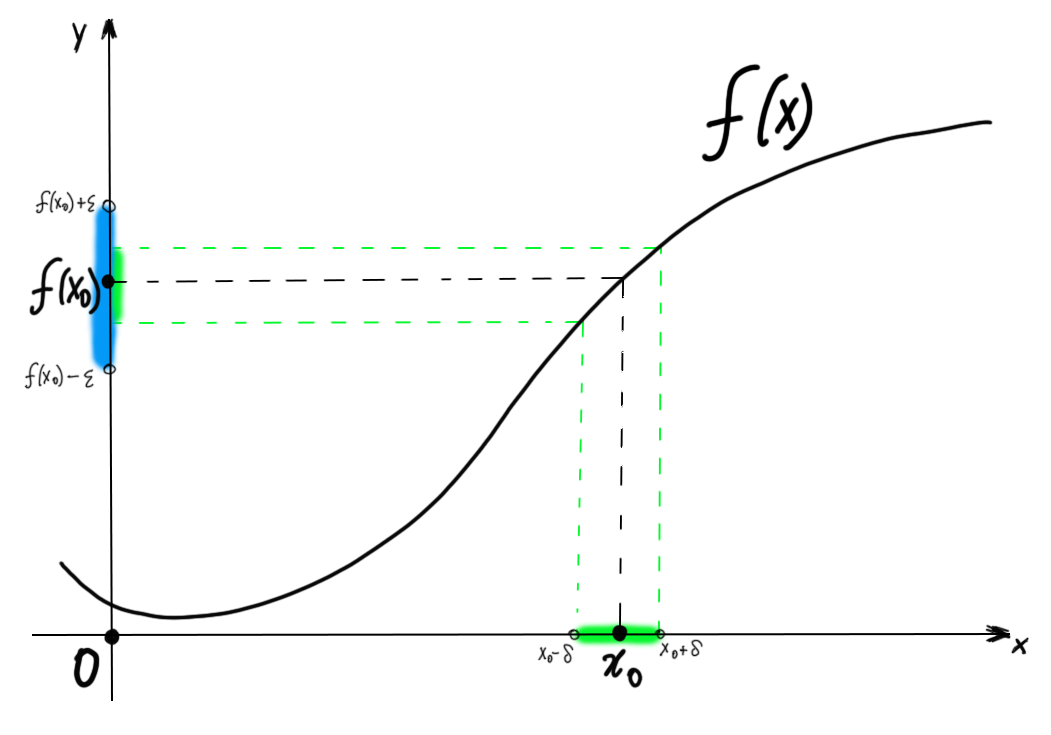
\includegraphics[width=0.7\linewidth]{images/continous.png}
    \caption{Пример графика непрерывной функции; для любой \textcolor{cyan}{$\varepsilon$-окрестности} точки $f(x_0)$ найдётся \textcolor{green}{$\delta$-окрестность} точки $x_0$, такая, что функция $f$ полностью отобразит эту \textcolor{green}{$\delta$-окрестность} в \textcolor{cyan}{$\varepsilon$-окрестность}.} 
    \label{fig:enter-label}
\end{figure}

\begin{proof}[Доказательство Леммы \ref{contious_on_R}]~

(1) Пусть $f:\mathbb{R} \to \mathbb{R}$ -- непрерывная функция, тогда она непрерывна в любой точке. Тогда для любой точки $x_0$ выполняются условия определения \ref{def_of_cont_on_sets_on_R}, а так как согласно Лемме \ref{interval_is_open} множества $\mathscr{B}_\delta(x_0), \mathscr{B}_\varepsilon(f(x_0))$ открыты, то мы получаем включение $f\bigl(\mathscr{B}_\delta(x_0) \bigr) \subseteq \mathscr{B}_\varepsilon(f(x_0)).$

(2) Пусть теперь в точке $x_0 \in \mathbb{R}$ и для любой $\varepsilon$-окрестности точки $f(x_0)$ всегда можно найти такую $\delta$-окрестность точки $x_0$, что $ f\bigl(\mathscr{B}_{\delta}(x_0) \bigr) \subseteq \mathscr{B}_{\varepsilon}(f(x_0))$. 

Рассмотрим теперь произвольную окрестность $\mathscr{W}(f(x_0))$ точки $f(x_0)$. Так как $\mathscr{W}(f(x_0))$ -- открытое в $\mathbb{R}$ множество, то согласно  определению \ref{open_in_R} существует такое $\varepsilon$-окрестность $\mathscr{B}_\varepsilon(f(x_0))$ точки $f(x_0)$, что $\mathscr{B}_\varepsilon(f(x_0)) \subseteq \mathscr{W}(f(x_0))$. Согласно предположению мы теперь можем найти $\delta$-окрестность точки $x_0$, что $ f\bigl(\mathscr{B}_{\delta}(x_0) \bigr) \subseteq \mathscr{B}_{\varepsilon}(f(x_0))$. Таким образом, мы получаем цепочку включений
\[
 f\bigl(\mathscr{B}_{\delta}(x_0) \bigr) \subseteq \mathscr{B}_{\varepsilon}(f(x_0)) \subseteq \mathscr{W}(f(x_0)),
\]
\textit{т.е.,} $f\bigl(\mathscr{B}_{\delta}(x_0) \bigr) \subseteq \mathscr{W}(f(x_0))$. Так как  (см. лемму \ref{interval_is_open}, $\mathscr{B}_{\delta}(x_0)$ -- открыто, то мы получаем, что для любого открытого множества $\mathscr{W}(f(x_0))$ мы нашли такое открытое $\mathscr{B}_{\delta}(x_0)$, что $f\bigl(\mathscr{B}_{\delta}(x_0) \bigr) \subseteq \mathscr{W}(f(x_0))$, а это и означает непрерывность (см. определение \ref{def_of_cont_on_sets_on_R}). Это завершает доказательство.
\end{proof}

\begin{corollary}\label{reform_of_cont}
  Для того, чтобы функция $f:\mathbb{R} \to \mathbb{R}$ была непрерывной в точке $x_0$, необходимо и достаточно, чтобы для всякого $\varepsilon>0$ существовал такой $\delta >0$, что из $|x-x_0|<\delta$ следует $|f(x)-f(x_0)|<\varepsilon$.    
\end{corollary}

\begin{proof}
    Действительно, для этого мы положим, что $\mathscr{W}(f(x_0)) = (f(x_0)-\varepsilon, f(x_0) + \varepsilon)$ и $\mathscr{U}(x_0) = (x_0-\delta,x_0 + \delta)$ в формулировке леммы \ref{contious_on_R}.
\end{proof}

\begin{figure}[h!]
    \centering
    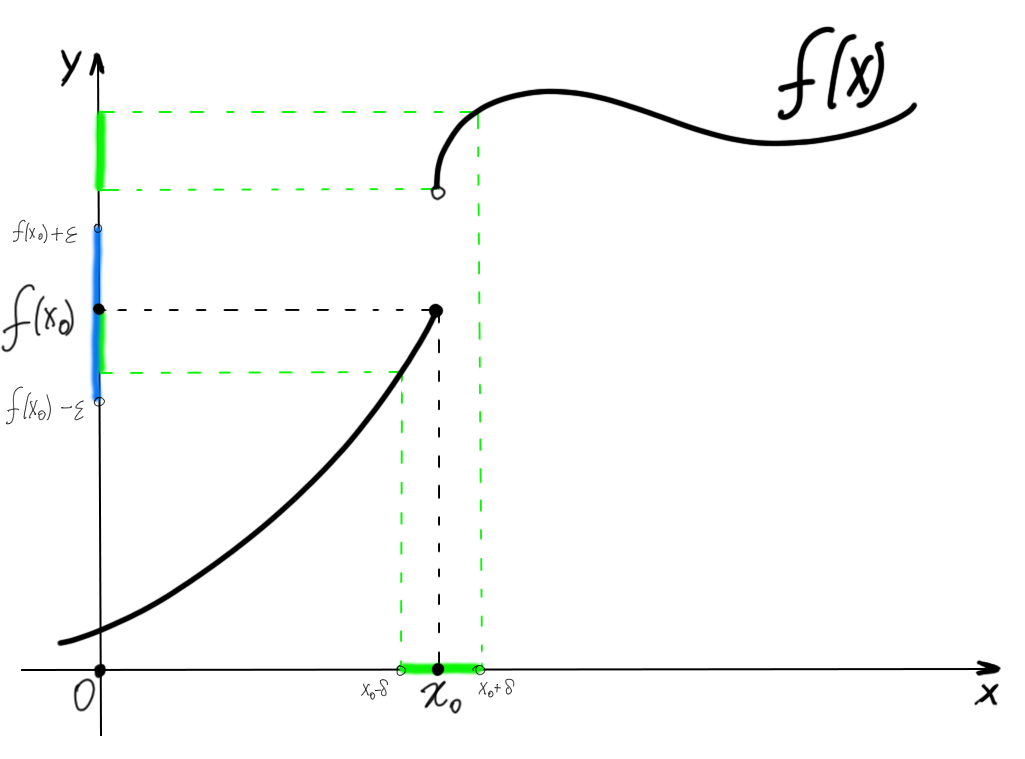
\includegraphics[width=0.7\linewidth]{images/non_continous.png}
    \caption{Пример графика функции которая не является непрерывной в точке $x_0$; мы нашли такую \textcolor{cyan}{$\varepsilon$-окрестность} точки $f(x_0)$, что никакая \textcolor{green}{$\delta$-окрестность} точки $x$ целиком не отображается в эту \textcolor{cyan}{$\varepsilon$-окрестность}.}
    \label{fig:enter-label}
\end{figure}

\begin{remark}\label{not_continous}
Тогда если $f:\mathbb{R} \to \mathbb{R}$ не является непрерывной функцией  в точке $x_0$, то можно найти такую $\varepsilon$-окрестность $\mathscr{B}_\varepsilon(f(x_0))$ точки $f(x_0)$, что не существует $\delta$-окрестности $\mathscr{B}_\delta(x_0)$ точки $x_0$, что $f(\mathscr{B}_\delta(x_0)) \not \subseteq \mathscr{B}_\varepsilon(f(x_0))$. 
\end{remark}



\begin{example}\label{x^2_is_continous}
    Пусть $f(x) = x^2$. Покажем, что эта функция непрерывна. Возьмём произвольную точку $x_0 \in \mathbb{R}$ и покажем, что $f$ непрерывна в этой точке. Согласно следствию \ref{reform_of_cont}, нам нужно для любого $\varepsilon>0$ найти такое $\delta >0$, что из неравенства $|x- x_0|< \delta$ будет следовать неравенство $|x^2 - x_0^2|<\varepsilon.$

    Имеем
    \begin{eqnarray*}
        |f(x)- f(x_0)| &=& |x^2 - x_0^2| \\
        &=& |(x-x_0)(x+x_0)| \\
        &=& |x-x_0| \cdot |x+x_0| \\
        &=& |x-x_0|\cdot \left| (x-x_0) + 2x_0 \right| \\
        &\le& |x-x_0| \cdot \left( |x-x_0| + 2 |x_0| \right).
    \end{eqnarray*}

Поэтому если $|x-x_0|<\delta$ и если мы потребуем, чтобы $\delta (\delta + 2|x_0|)<\varepsilon$, то из неравенства $|x-x_0|<\delta$ будет следовать неравенство $|f(x)- f(x_0)| < \varepsilon$, что и доказывает непрерывность этой функции. 
\end{example}

\begin{example}\label{x^2sin(1x)}
Покажем, что функция $f:\mathbb{R} \to \mathbb{R}$
    \[
    f(x) = \begin{cases}
         x^2 \sin \frac{1}{x}, & x \ne 0, \\
         0, & x =0
     \end{cases}
    \]
непрерывнa в точке $0$.

Это значит, что для любого $\varepsilon >0$ мы должны найти такую $\delta >0$, что из неравенства $|x|<\delta$ будет следовать $|{f}(x) - {f}(0)| = |f(x)| <\varepsilon.$

Имеем 
    \[
    \left|{f}(x) -{f}(0)\right| = \left|x^2 \sin \frac{1}{x} - 0 \right| = \left|x^2 \sin \frac{1}{x}\right| \le |x^2| = x^2,
    \]
поэтому если $x^2 <\varepsilon$, \ie $-\sqrt{ \varepsilon} <x < \sqrt{\varepsilon}$, то и $|{f}(x) - {f}(0)| <\varepsilon$. Значит, для любого $0 < \delta < \sqrt{\varepsilon}$ из неравенства $|x|<\delta$ вытекает неравенство $|{f}(x) - {f}(0)|$, что и доказывает непрерывность в точке $0.$
\end{example}

\subsection{Критерий непрерывности}


\begin{theorem}\label{preimage_of_open}
Пусть $X,Y \subseteq \mathbb{R}$ -- непустые подмножества на прямой. Функция $f:X \to Y$ непрерывна тогда и только тогда, когда прообраз любого открытого множества в $Y$ является открытым множеством в $X.$
\end{theorem}
\begin{proof}~

(1) Пусть $f:X \to Y$ -- непрерывная функция. Возьмём произвольное открытое множество $\mathscr{W} \subseteq Y$ и покажем, что множество $f^{-1}(\mathscr{W})$ открыто в $X$.

Пусть $x \in f^{-1}(\mathscr{W})$, тогда существует такой $y \in \mathscr{W}$, что $f(x) = y$. Далее, так как $\mathscr{W}$ является открытым множеством в $Y$, при этом $y\in \mathscr{W}$, $f(x) = y$, и $f$ -- непрерывно в $x$, то согласно определению \ref{def_of_cont_on_sets_on_R}, найдётся такое открытое в $X$ множество $\mathscr{U} \subseteq X$, что $x \in \mathscr{U}$ и $f(\mathscr{U}) \subseteq \mathscr{W}.$ Тогда согласно предложению \ref{good_for_maps}, получаем включение
\[
 f^{-1}(f(\mathscr{U})) \subseteq f^{-1}(\mathscr{W}),
\]
наконец, согласно предложению \ref{good_for_preimage}, имеем
\[
 \mathscr{U} \subseteq f^{-1}(f(\mathscr{U})) \subseteq f^{-1}(\mathscr{W}).
\]

Итак, мы получили следующее. Для любой точки $x \in f^{-1}(\mathscr{W})$ мы нашли такое открытое в $X$ множество $\mathscr{U}$, что

\[
 x \in \mathscr{U} \subseteq f^{-1}(f(\mathscr{U})) \subseteq f^{-1}(\mathscr{W}).
\]
но тогда согласно предложению \ref{open_via_open} множество $f^{-1}(\mathscr{W})$ -- открыто в $X.$


(2) Пусть прообраз любого открытого множества в $Y$ есть открытое множество в $X$. Пусть $f(x) = y$ и пусть $y \in \mathscr{W}$, где $\mathscr{W}$ -- открытое множество в $Y$. Тогда $x \in f^{-1}(\mathscr{W})$, а так как мы предположили, что множество $f^{-1}(\mathscr{W})$ -- открыто в $X$, то согласно предложению \ref{open_via_open}, найдётся такое открытое множество $\mathscr{U}$ в $X$, что
\[
 x \in \mathscr{U} \subseteq f^{-1}(\mathscr{W}).
\]

Так как $\mathscr{U} \subseteq f^{-1}(\mathscr{W})$, то согласно предложению \ref{good_for_maps}, имеем $f(\mathscr{U}) \subseteq f(f^{-1}(\mathscr{W}))$. Наконец, согласно предложению \ref{good_for_preimage}, $f(f^{-1}(\mathscr{W})) \subseteq \mathscr{W}$.

Итак, мы получили, что для любой точки $y\in Y$ и любого открытого множества $\mathscr{W}$ в $Y$ мы нашли такое открытое множество $\mathscr{U}$ в $X$, что 
\[
f(\mathscr{U}) \subseteq f(f^{-1}(\mathscr{W})) \subseteq \mathscr{W},
\]
\textit{т.е.} $f(\mathscr{U}) \subseteq \mathscr{W}$, но согласно определению \ref{def_of_cont_on_sets_on_R}, это и означает непрерывность в точке $x$, а так как $x$ -- произвольная точка, то это означает непрерывность на всём $X$.
\end{proof}

\begin{mydangerr}{\bf!}
    Следует заметить, что образ открытого множества при непрерывном отображении, вообще говоря, \textbf{не будет} открытым множеством.
\end{mydangerr}


\begin{example}
    Вернёмся к примеру \ref{x^2_is_continous}, $f:\mathbb{R} \to \mathbb{R}$, $f(x) = x^2$. Мы показали, что $f$ -- непрерывная функция. Если мы рассмотрим теперь открытый интервал $(-1,1)$, то его образом при $f$ будет множество $[0,1)$, которое не открыто в $\mathbb{R}$ (см. Пример \ref{(a,b)c(open}).
\end{example}



\begin{theorem}\label{comp_of_continous_on_R}
 Пусть $X,Y,Z \subseteq \mathbb{R}$ -- непустые подмножества  и пусть $f:X \to Y$, $g:Y \to Z$ -- функции.
\[
 \xymatrix{
 X \ar@{->}[r]^f \ar@{->}[rd]_{g\circ f} & Y \ar@{->}[d]^g \\
 & Z 
 }
\]
Если $f$ непрерывная в точке $x_0$ и $g$ непрерывная в точке $f(x_0)$, то функция $h = g \circ f$ непрерывная в точке $x_0.$ Если $f$ непрерывна на всём $X$ и $g$ непрерывная на всём $Y$, то $h$ непрерывная на всём $X.$
\end{theorem}
 \begin{proof}
Пусть $\mathscr{W}$ -- окрестность точки $h(x_0) =  g(f(x_0))$. Тогда из предположения о непрерывности (см. Определение \ref{def_of_cont_on_sets_on_R}) найдётся окрестность $\mathscr{V}$ точки $f(x_0)$, такая что
\[
 g(\mathscr{V}) \subseteq \mathscr{W}.
\]

С другой стороны, так как $f$ -- непрерывна в точке $x_0$, тогда (см. Определение \ref{def_of_cont_on_sets_on_R}) для этой же окрестности $\mathscr{V}$ существует окрестность $\mathscr{U}$ точки $x_0$, такая что
\[
 f(\mathscr{U}) \subseteq \mathscr{V}.
\]

Воспользовавшись теперь (\ref{A<B->F(A)<F(B)}), мы получаем 
\[
 g(f(\mathscr{U})) \subseteq g(\mathscr{V)} \subseteq \mathscr{W},
\]
но это и означает (см. Определение \ref{def_of_cont_on_sets_on_R}) что функция $h = g \circ f$ -- непрерывна в точке $x_0$.

Второе утверждение, очевидно, следует из первого. 
 \end{proof}


\begin{corollary}\label{restriction_on_R}
    Если $f:X \to Y$ непрерывное в точке $x_0$ функция, и $A \subseteq X$, $A \ni x_0$, то сужение $f|_A:=f \circ \mathrm{in}_A$ также непрерывно в $x_0,$ где $\mathrm{in}_A:A \hookrightarrow X$ -- вложение.
\end{corollary}
\begin{proof}
    На самом деле, $f$ непрерывно в $x_0$ по условию, а $\mathrm{in}_A$ непрерывно в любой точке $a \in A$ (потому что это тождественная функция), тогда из предыдущей теоремы и следует утверждение.
\end{proof}




\section{Лекция \#13. Пределы}

\subsection{Основное определение}

\begin{definition}\label{the_main_def_of_limit_on_R}
Пусть $X, Y \subseteq \mathbb{R}$ -- непустые подмножества, $x_0 \notin X$, но $x_0 \in \overline{X}$. Пусть далее $f: X \to Y$. Мы будем говорить, что $f(x)$ \textit{имеет предел $y_0 \in Y$ при $x \in X$, стремящемся к $x_0$ (или $y_0$ есть предел функции $f$ в точке $x_0 \in \overline{X}$ по множеству $X$}), если функция $\overline{f}:X \cup \{x_0\} \to Y$, определённая условиями
    \[
     \overline{f}(x) = \begin{cases}
         f(x), & x \in X, \\
         y_0, & x = x_0,
     \end{cases}
    \]
    непрерывна в точке $x_0$.
\end{definition}

В этом случае, мы пишем
\[
 y_0 := \lim_{x\to x_0, x \in X} f(x).
\]

\begin{mydanger}{\bf{!}}
    Если $x_0 \in X$, то мы пользуемся той же терминологией и теми же обозначениями как и в случае, когда функция $f$ непрерывна в точке $x_0$, причём $y_0:=f(x_0).$
\end{mydanger}

\begin{example}
Пусть $X = \mathbb{R}\setminus\{0\}$, $Y = \mathbb{R}$, а функция $f:X\to Y$ задана следующим образом:
\[
 f(x): = x^2 \sin \frac{1}{x}.
\]

\begin{figure}[h!]
    \centering
    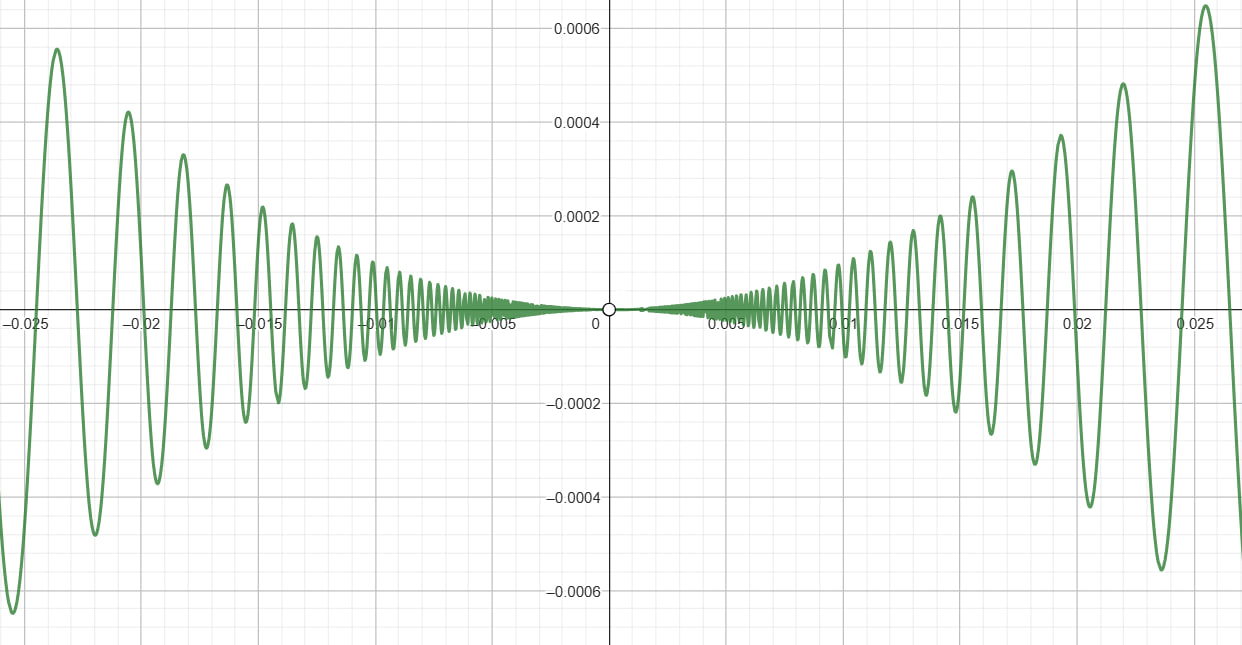
\includegraphics[width=1\linewidth]{images/x2sin.jpg}
    \caption{График функции $f(x) = x^2 \sin \frac{1}{x}$. Видно, что если мы положим $f(0):=0$, то мы получим непрерывную функцию на всей прямой $\mathbb{R}$.}
\end{figure}


Ясно, что любая окрестность точки $x_0=0$ пересекается с множеством $X$, поэтому точка $x_0 = 0$ -- точка прикосновения для множества $X$, \textit{т.е.} $0 \in \overline{X}$.

Продолжим теперь нашу функцию на множестве $X\cup \{0\}$ следующим образом:
    \[
    \overline{f}(x) = \begin{cases}
         x^2 \sin \frac{1}{x}, & x \ne 0, \\
         0, & x =0
     \end{cases}
    \]
и покажем, что она непрерывнa в точке $x_0 =0$.

Это значит, что для любого $\varepsilon >0$ мы должны найти такую $\delta >0$, что из неравенства $|x|<\delta$ будет следовать $|\overline{f}(x) -\overline{f}(0)| = |\overline{f}(x)| <\varepsilon.$

Имеем 
    \[
    \left|\overline{f}(x) -\overline{f}(0)\right| = \left|x^2 \sin \frac{1}{x} - 0 \right| = \left|x^2 \sin \frac{1}{x}\right| \le |x^2| = x^2,
    \]
поэтому если $x^2 <\varepsilon$, \ie $-\sqrt{ \varepsilon} <x < \sqrt{\varepsilon}$, то и $|\overline{f}(x) - \overline{f}(0)| <\varepsilon$. Значит, для любого $0 < \delta < \sqrt{\varepsilon}$ из неравенства $|x|<\delta$ вытекает неравенство $|\overline{f}(x) - \overline{f}(0)|$, что и доказывает непрерывность в точке $0.$ 

Поэтому имеем
\[
\lim_{x \to 0, x \in X}f(x) = 0  
\]
\begin{flushright}
    $\square$
\end{flushright}
\end{example}


Вспомнив определение непрерывности (см. Определение \ref{def_of_cont_on_sets_on_R}) и точки прикосновения (см. Определение \ref{limit_point}), определение предела можно переформулировать следующими двумя эквивалентными способами:

\begin{definition}\label{lim_via_neighberhoods}
Когда говорят, что функция $f: X \to Y$ имеет предел $y_0$ при $x \in X$, стремящимся к $x_0$, и при этом пишут
\[
 \lim_{x \to x_0, x \in X}f(x) = y_0
\]
то это означает, что для каждого открытого в $Y$ множества $\mathscr{W}$, $y_0 \in \mathscr{W}$ найдётся такое открытое в $\mathbb{R}$ множество $\mathscr{U}$, что $x_0 \in \mathscr{U}$ и $f(\mathscr{U}\cap X) \subseteq \mathscr{W}$. 
\end{definition}

\begin{mydanger}{\bf{!}}
    Так как $x_0 \in \overline{X}$, то множество $X \cap \mathscr{U}$ никогда не пусто.
\end{mydanger}

\begin{definition}\label{def_for_cont_via_d-e_on_R}
Сказать, что функция $f: X \to Y$ имеет предел $y_0$ при $x \in X$, стремящимся к $x_0$, и при этом написать
\[
 \lim_{x \to x_0, x \in X}f(x) = y_0,
\]
это то же самое, что сказать, что для каждого $\varepsilon>0$ можно найти такое $\delta >0$, что из $x \in X$ и $|x-x_0|<\delta$ следует $|f(x) - f(x_0)|<\varepsilon.$
\end{definition}

\begin{proposition}
 Функция может иметь лишь один предел по множеству $X$ в данной точке $x_0 \in \overline{X}.$
\end{proposition}
\begin{proof}
    Пусть  $\lim_{x \to x_0, x \in X}f(x) = y_0$ и $\lim_{x \to x_0, x \in X}f(x) = y_0'$, при этом $y_0 \ne y_0'$. Тогда согласно Определению \ref{def_for_cont_via_d-e_on_R}, мы для любого $\varepsilon>0$ можем найти такие $\delta, \delta' >0$, что из неравенств $|x-x_0|< \delta$, $|x-x_0|<\delta'$ будут следовать неравенства $|f(x) - y_0|, |f(x)-y_0'|<\varepsilon.$

Имеем
\begin{eqnarray*}
    |y_0 - y_0'| &=& |y_0 - f(x) + f(x) - y_0'| \\
    &=& |(y_0-f(x)) + (f(x) - y_0')| \\
    &\le & |f(x) - y_0| + |f(x) - y_0'| \\
    &<& 2 \varepsilon,
\end{eqnarray*}
\textit{т.е.} расстояние между фиксированными точками $y_0,y_0' \in Y$ может быть любым, что невозможно, если $y_0 \ne y_0'.$
\end{proof}





\subsection{Критерий непрерывности в терминах предела}

Из определения предела вытекает:

\begin{theorem}[{Критерий непрерывности}]\label{criteria_of_continous}
Функция $f: X \to Y$ непрерывна в точке $x_0 \in X$, являющейся точкой прикосновения множества $X\setminus\{x_0\}$, тогда и только тогда, когда
\[
f(x_0) = \lim_{x \to x_0, x\in X \setminus \{x_0\}}f(x)
\]
\end{theorem}
\begin{proof}
    Это лишь пересказ определения предела (см. Определение \ref{the_main_def_of_limit_on_R}).
\end{proof}

\begin{theorem}\label{limit_for_any_subset}
    Пусть $y_0 = \lim_{x \to x_0, x \in X} f(x)$. Тогда для каждого подмножества $A \subseteq X$, для которого $x_0 \in \overline{A}$, $y_0 = \lim_{x \to x_0, x \in B}f(x)$.
\end{theorem}

\begin{proof}
    Это сразу следует из определения предела (см. Определение \ref{the_main_def_of_limit_on_R}) и следствия \ref{restriction_on_R}.
\end{proof}





\begin{theorem}\label{lim_of_composition_on_R}
Пусть $X,Y,Z \subseteq \mathbb{R}$ -- непустые множества, пусть имеем функции 
\[
 \xymatrix{
 X \ar@{->}[r]^f \ar@{->}[rd]_{g\circ f} & Y \ar@{->}[d]^g \\
 & Z
 }
\]
Тогда, если
\[
 \lim_{x\to x_0, x\in X}f(x) = y_0,
\]
и функция $g$ -- непрерывна в точке $y_0$, то
\[
 g(y_0) = \lim_{x \to x_0, x \in X} (g \circ f)(x).
\]     
\end{theorem}
\begin{proof}
    Это сразу следует из определения предела (см. Определение \ref{the_main_def_of_limit_on_R}) и теоремы \ref{comp_of_continous_on_R}.
\end{proof}

\begin{mydanger}{\bf{!}}
    В случае, когда $X = \mathbb{R}$, мы будем вместо $\lim_{x \to x_0, x \in \mathbb{R}}f(x)$ писать $\lim_{x \to x_0}f(x).$
\end{mydanger}


\subsection{Окрестность бесконечности}\label{neighborhood_of_infinity}

Мы сейчас довольно-таки ``окольным путём'' приблизимся к понятию гомеоморфизма между топологическими пространствами. Делаем мы это лишь для того, чтобы не перегрузить читателя большим количеством новых терминов, которые потом не будут так часто использоваться.

\begin{construction}\label{con_of_induced_topology}
 Пусть дано некоторое непустое подмножество $X\subseteq \mathbb{R}$ и произвольное множество $S$. Допустим, что у нас есть биекция $\varphi:X \to S$, тогда мы можем снабдить это абстрактное множество $S$ топологией, наследованной из множества $X$, а именно будем считать $\mathscr{V} \subseteq S$ открытым тогда и только тогда, когда $\varphi^{-1}(\mathscr{V}) \subseteq X$ -- открыто в $X.$
\end{construction}

\begin{mydangerr}{\bf !}
    Если рассматривать абстрактные топологические пространства, то в таком случае непрерывное отображение между ними определяют как такое отображение, прообраз каждого подмножества которого открыт. Фактически, то что мы определили, это специально построили такую топологию на $S$, чтобы $\varphi$ было непрерывным.
\end{mydangerr}


\begin{definition}
 Обозначим через $\overline{\mathbb{R}}$ множество, являющееся объединением $\mathbb{R}$ и двух новых элементов, обозначаемых символами $+\infty$ и $-\infty$ (=\textit{бесконечные точки}), \textit{т.е}
\[
 \overline{\mathbb{R}}: = \mathbb{R}\cup \{-\infty\} \cup \{+\infty\}.
\]
\end{definition}

\begin{mydanger}{\bf !}
Об этих символах следует думать как о бесконечно удалённых точках. Самый более или менее подходящий пример — это понятие горизонта, которого никогда не достигнуть.
\end{mydanger}

\begin{figure}
    \centering
    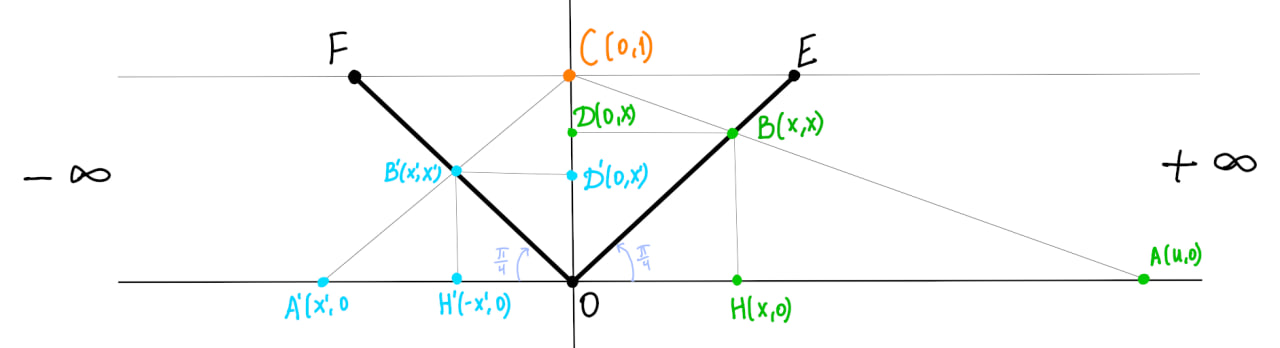
\includegraphics[width=1\linewidth]{images/infty.jpg}
    \caption{Схема отображения $\varphi: [-1,1] \to \overline{R}$; сам отрезок $[-1,1]$ тут представлен ломаной $FOE$. Тонкие линии на рисунке показывают, куда отображаются точки отрезка; $E \mapsto +\infty$, $B \mapsto A$, $B' \mapsto A'$, $F \mapsto -\infty$. Ясно, что это биекция.}
    \label{infnty_picture}
\end{figure}

Наша цель — это ввести топологию на множестве $\overline{\mathbb{R}}$. Мы будем делать это исходя из того, что мы знаем топологию на отрезке. Для этого нам понадобится биекция $\varphi: [-1,1] \to \overline{\mathbb{R}}$ и Конструкция \ref{con_of_induced_topology}.

Напомним (см. Теорема \ref{open_in_K}), что открытые множества в $[-1,1]$ это множества вида $\mathscr{U} \cap [-1,1]$, тогда, например, окрестностью точки $1$ будет множество $(\alpha, 1]$, где $-1 \le \alpha<1$.

\begin{construction}\label{construction_of_bijection}
Определим отображение $\varphi: [-1,1] \to \overline{\mathbb{R}}$, следующим образом
\[
 \varphi(x): = \begin{cases}
     \frac{x}{1-|x|}, & -1<x<1,\\
     + \infty, &x = 1, \\
     -\infty, & x=-1
 \end{cases}
\]
схема которого изображена на Рис.\ref{infnty_picture}. Обратное отображение $\varphi^{-1}: \overline{\mathbb{R}} \to [-1,1]$ выглядит следующим образом
\[
\varphi^{-1}(x): = \begin{cases}
    \frac{x}{1+ |x|}, & x \in \mathbb{R},\\
    1, & x = + \infty,\\
    -1, & x = - \infty.
\end{cases}
\]
\end{construction}

\begin{lemma}\label{x<y->f(x)<f(x)}
    Если $x,y\in \mathbb{R}$, то $x\le y$ тогда и только тогда, когда $\varphi^{-1}(x) \le \varphi^{-1}(y)$.
\end{lemma}
\begin{proof}
Рассмотрим все возможные случаи.

(1) Пусть $x,y \ge 0$, тогда $|x| =x$ и $|y| = y$.

Имеем
\begin{eqnarray*}
    x \le y &\Longleftrightarrow& x+ xy \le y + xy \\
    & \Longleftrightarrow& x (1 + y) \le y(1 + x)\\
    &\Longleftrightarrow& x(1+ |y|) \le y (1+ |x|)\\
    &\Longleftrightarrow& \frac{x}{1+|x|} \le \frac{y}{1+|y|}\\
    &\Longleftrightarrow& \varphi^{-1}(x) \le \varphi^{-1}(y).
\end{eqnarray*}

(2) Пусть $x <0$, $y \le 0$, тогда $|x|  =- x$ и $|y| = y$, а также $xy < 0$.

Имеем

\begin{eqnarray*}
    x \le y &\Longleftrightarrow& x + xy \le  y+xy \le y -xy \\
    &\Longleftrightarrow& x+xy \le y - xy\\
    &\Longleftrightarrow& x(1+y) \le y(1-x) \\
    &\Longleftrightarrow& \frac{x}{1-x} \le \frac{y}{1+y}\\
    &\Longleftrightarrow& \varphi^{-1}(x) \le \varphi^{-1}(y).
\end{eqnarray*}

(3) Пусть $x,y < 0$ и $x\le y$, тогда $|x| = -x$, $|y| = -y$, $xy >0$.

Имеем

\begin{eqnarray*}
    x \le y &\Longleftrightarrow& x-xy \le y - xy \\
    &\Longleftrightarrow & x(1-y) \le y(1-x) \\
    &\Longleftrightarrow& \frac{x}{1-x} \le \frac{y}{1-y}\\
    &\Longleftrightarrow& \frac{x}{1+|x|} \le \frac{y}{1+ |y|} \\
     &\Longleftrightarrow& \varphi^{-1}(x) \le \varphi^{-1}(y).
\end{eqnarray*}

Это завершает доказательство.
\end{proof}

\begin{construction}
 На $\overline{\mathbb{R}}$ введём отношение порядка, по определению считая неравенство $x \le y$ эквивалентным неравенству $\varphi^{-1}(x) \le \varphi^{-1}(y)$. Легко проверить, что, когда $x,y \in \mathbb{R}$, это отношение порядка есть обычное отношение порядка на $\mathbb{R}$ и что, кроме того, для любого $x\in \mathbb{R}$ мы имеем $- \infty < x < \infty.$    
\end{construction}

\begin{mydanger}{\bf !}
    Действительные числа называются также \textit{конечными} элементами $\overline{\mathbb{R}}.$ 
\end{mydanger}~

Таким образом, согласно конструкции \ref{con_of_induced_topology} и теореме \ref{open_in_K}, получаем следующее

\begin{definition}
 Открытые множества в $\overline{R}$ — это открытые множества $\mathbb{R}$, а также множества вида $\varphi(\mathscr{U}\cap [-1,1])$, таким образом, окрестностями точек $-\infty,+\infty$ могут служить, например, множества $[-\infty, a)$, $(b,+\infty]$, соответственно, где $a,b \in \mathbb{R}$.  
\end{definition}


\begin{lemma}\label{niegh_of_infty_on_R}
  Точки $-\infty, + \infty$ -- точки прикосновения для $\mathbb{R} \subseteq \overline{\mathbb{R}}.$
 \end{lemma}
 \begin{proof}
Мы докажем это утверждение для $+\infty$, так как для $-\infty$ оно доказывается аналогично.

Итак, пусть $\mathscr{W}$ -- окрестность точки $+\infty$, тогда, согласно конструкциям \ref{con_of_induced_topology}, \ref{construction_of_bijection}, существует открытое в $[-1,1]$ множество $\mathscr{U}(1)$, содержащее точку $1$, такое, что $\mathscr{W} = \varphi^{-1}(\mathscr{U}(1))$.  

Но, согласно определению \ref{e-neigh_in_A}, множество $\mathscr{U}(1)$ содержит в себе множество вида $(a,1]$, где $-1\le a <1$. Далее, согласно свойству (\ref{A<B->F(A)<F(B)}), получаем, 
\[
 (a,1] \subseteq \mathscr{U}(1) \Longrightarrow \varphi((a,1]) \subseteq \varphi(\mathscr{U}(1)) = \mathscr{W},
\]
наконец, согласно конструкции \ref{construction_of_bijection} и лемме \ref{x<y->f(x)<f(x)}, получаем
\[
 \varphi((a,1]) = \left.\left( \frac{a}{1-|a|}, +\infty\right.\right],
\]
\textit{т.е.} $\left.\left( a', +\infty\right.\right] \subseteq \mathscr{W}$, где $a' = \frac{a}{1-|a|}$. Итак, любая окрестность точки $+\infty$ содержит в себе множество вида $(a',\infty]$, где $a' \in \mathbb{R}$. Но так как $(a',\infty] \cap \mathbb{R} \ne \varnothing$, то это и означает, что $+\infty$ -- точка прикосновения. 
 \end{proof}

\subsection{Символ $\lim\limits_{x \to \infty}$ и предел последовательности}

Пусть теперь $X,Y \subseteq \overline{\mathbb{R}}$ -- непустые подмножества и пусть $f: X \to Y$ -- функция. 

\begin{remark}\label{about_infty}
Так как (см. Лемму \ref{niegh_of_infty_on_R}) любая окрестность точки $+\infty$ (\textit{соотв.} точки $-\infty$) содержит в себе множество $(a,+\infty]$ (\textit{соотв.} множество $[-\infty, a)$), то получаем
\begin{enumerate}
    \item[] во-первых, если $+\infty$ (\textit{соотв.} $-\infty$) -- точка прикосновения для $X$, то это значит что для любого $x \in X$ существует, такой $x' \in X$, что $x<x'$ (\textit{соотв.} $x'<x$),
    \item[] во-вторых, если $f$ -- непрерывна в точке $-\infty$, то это значит, что для любого открытого в $Y$ множества $\mathscr{W}(y_0)$, содержащее точку $y_0 = f(-\infty)$ найдётся такое число $a \in X$, что для всех $x'\in X$, с условием $x'< a$ верно то, что $f(x') \in \mathscr{W}(y_0)$,
    \item[] аналогично, если $f$ -- непрерывна в точке $+\infty$, то это значит, что для любого открытого в $Y$ множества $\mathscr{W}(y_0)$, содержащее точку $y_0 = f(+\infty)$ найдётся такое число $a \in X$, что для всех $x'\in X$, с условием $x'>a$ верно то, что $f(x') \in \mathscr{W}(y_0)$.
\end{enumerate}    
\end{remark}


Рассмотрим теперь множество натуральных чисел $\mathbb{N} \subseteq \mathbb{R}$, тогда, согласно теореме \ref{open_in_K}, любое открытое в $\mathbb{N}$ множество это множество вида $\mathscr{U} \cap \mathbb{N}$.

Это значит, что все натуральные числа в любом открытом множестве $\mathscr{U} \subseteq \mathbb{R}$ и есть открытое множество в $\mathbb{N}$, \textit{т.е.,} любой набор точек из $\mathbb{N}$ образует открытое множество в $\mathbb{N}$. В частности одноточечное множество $\{n\}$ -- открыто в $\mathbb{N}.$

\begin{mydangerr}{\bf !}
    Аналогично рассуждая (используя предложение \ref{closed_in_A_if}), получаем что любой набор точек из $\mathbb{N}$ -- замкнут. Таким образом, в $\mathbb{N}$ любое подмножество как замкнуто так и открыто одновременно и более того, любая точка тоже обладает этим свойством. 
\end{mydangerr}

\begin{theorem}\label{lim_of_seqence=contionous}
 Пусть дана последовательность $(x_n)$ каких-то элементов множества $X \subseteq \mathbb{R}$ и пусть $\lim_{n\to \infty}x_n =a$ в смысле определения \ref{limit_of_seqeunce}, тогда функция $\m{x}: \mathbb{N} \to X$ определённая условием
    \[
     \m{x}(n): =\begin{cases}
         x_n, & n \ge 1\\
         a, & n = +\infty
     \end{cases}
    \]
    непрерывна в точке $+\infty$, а значит $\lim_{n \to +\infty\, n \in \mathbb{N}}\m{x}(n) = a$ в смысле определения \ref{the_main_def_of_limit_on_R}. И более того, верно и обратное утверждение.
\end{theorem}
\begin{proof}
    Это сразу следуют из определения \ref{limit_of_seqeunce}, определения \ref{the_main_def_of_limit_on_R} и замечания \ref{about_infty}.
\end{proof}





\section{Лекция \#14. Определение предела в терминах предал последовательностей и $o$-символика}

\subsection{Предел функции в терминах предела последовательностей}

Мы сейчас выведем ещё одно очень полезное свойство предела функции, которое принято называть \textit{определением предела функции по Гейне\footnote{Генрих Эдуард Гейне (нем. Heinrich Eduard Heine; 15 марта 1821, Берлин, Германия — 21 октября 1881, Галле, Германия) — немецкий математик, профессор. Ученик Дирихле.}}.

\begin{lemma}\label{choice_of_seqeunce_on_R}
Пусть $A\subseteq \mathbb{R}$ -- непустое множество, тогда для любой точки $a \in \overline{A}$ существует такая последовательность $(a_n)$ точек из $A$, что $a = \lim_{n \to \infty} a_n$.
\end{lemma}

\begin{proof}
 Так как $a$ -- точка прикосновения, то для любой её $\varepsilon$-окрестности $(a-\varepsilon, a+\varepsilon)$ имеем $A \cap (a-\varepsilon, a+\varepsilon) \ne \varnothing$. Другими словами любая её $\varepsilon$-окрестность $(a-\varepsilon, a+\varepsilon)$ содержит хотя бы одну точку из $A$. В частности,  для любого $n\ge 1$, пологая $\varepsilon: = \frac{1}{n}$, получаем 
 \[
  \left(a - \frac{1}{n}, a+ \frac{1}{n} \right) \cap A \ne \varnothing.
 \]

Тогда для каждого $n\ge 1$ мы можем выбрать\footnote{так как у нас счётный набор множество, то это можно сделать не прибегая к помощи аксиомы выбора.} $a_n \in   \left(a - \frac{1}{n}, a+ \frac{1}{n} \right) \cap A$.

Покажем, что $\lim_{n \to \infty} a_n = a$. Действительно, пусть $n<m$, и мы имеем тогда 
\[
 a_n \in   \left(a - \frac{1}{n}, a+ \frac{1}{n} \right) \cap A \mbox{ и } a_m \in   \left(a - \frac{1}{m}, a+ \frac{1}{m} \right) \cap A.
\]

Получаем
\begin{eqnarray*}
    |a_n -a_m| &=& |a_n - a + a - a_m| \\
    &=& |(a_n -a) + (a - a_m)| \\
    &\le & |a_n - a| + |a- a_m| \\
    &<& \frac{1}{n} + \frac{1}{m} < \frac{2}{n}.
\end{eqnarray*}

Это означает, что все $a_n, a_{n+1}, \ldots \in \left(a-\frac{2}{n}, a+ \frac{2}{n}\right)$, \textit{т.е.,} последовательность $(a_n)$ -- фундаментальная (см. Определение \ref{foundamental_sequence}), а тогда согласно критерию Коши (см. Теорема \ref{Coshy}), $\lim_{n \to \infty} a_n = a.$ Это завершает доказательство.
\end{proof}

Следующий результат некоторые авторы принимают за определение предела функции, и говорят, что это определение функции по Гейне.

\begin{theorem}\label{lim=>for_any_sequence}
 Пусть $X,Y \subseteq \mathbb{R}$ -- непустые множества, $f: X \to Y$ -- функция, и $x_0 \in \overline{X}.$ Для того, чтобы $f$ имело предел $y_0 \in Y$ в точке $x_0$ по $X$, необходимо и достаточно, чтобы для каждой последовательности $(x_n)$ точек из $X$, сходящейся к $x_0$, последовательность $(f(x_n))$ сходилась к $y_0.$
\end{theorem}

\begin{proof}~

(1) Пусть $\lim_{x \to x_0, x \in X}f(x) = y_0$, тогда согласно определению предела \ref{the_main_def_of_limit}, функция $\overline{f}: X \cup \{x_0\} \to \mathbb{R}$,
\[
 \overline{f}(x) = \begin{cases}
     f(x), & x \ne x_0 \\
     y_0, & x = x_0
 \end{cases}
\]
является непрерывной в точке $x_0$.

Далее, так как $x_0 \in \overline{X}$, то согласно лемме \ref{choice_of_seqeunce_on_R}, мы можем выбрать такую последовательность $(x_n)$ точек из $X$, такая что $\lim_{n \to \infty }x_n = x_0$. Далее, согласно теореме \ref{lim_of_seqence=contionous}, функция $\m{x}: \mathbb{N} \to X$ определённая условиями
\[
 \m{x}(n): = \begin{cases}
     x_n, & n \ge 1,\\
     x_0, & n = +\infty
 \end{cases}
\]
-- непрерывна в точке $+\infty$, а значит и $\lim_{n \to +\infty,\, n \in \mathbb{N}}\m{x} = x_0$.

Итак, мы получаем коммутативную диаграмму
\[
 \xymatrix{
 \mathbb{N} \ar@{->}[r]^{\m{x}} \ar@{->}[rd]_{f \circ \m{x}} & X \ar@{->}[d]^f\\
 & Y
 }
\]
из которой видно, что функция $f\circ \m{x}$ это последовательность $(f(x_n))$, так как
\[
 (f\circ \m{x})(n):= f(\m{x}(n)) = f(x_n), \qquad n \ge 1.
\]

Более того по Теореме \ref{lim_of_composition_on_R}, эта последовательность $(f(x_n))$ имеет предел $y_0 = \overline{f}(x_0)$, что и доказывает необходимость.

(2) Будем доказывать от противного. Пусть для любой последовательности $(x_n)$ точек из $X$, $\lim_{n \to \infty} x_n = x_0$ имеем $\lim_{n \to \infty}f(x_n) = y_0$, но $y_0 \ne \lim_{x \to x_0, x\in X}f(x)$ в смысле определения \ref{the_main_def_of_limit_on_R}.

Тогда поучаем, что
\begin{enumerate}
    \item[] с одной стороны, $\lim_{n \to \infty} x_n = x_0$ влечёт (см. Определение \ref{lim_of_composition}), что, начиная с какого-то номера $N$, $|x_n - x_0| < \varepsilon$ для всех $n > N$,
    \item[] а с другой стороны $\lim_{x \to x_0, x\in X}f(x) \ne y_0$ означает, что $f(x)$ не является непрерывный в точке $x_0$.
\end{enumerate}

Из последнего тогда получаем, что существует такое $\varepsilon >0$, что для любого номера $n$ найдётся такая точка $x_n \in X$, удовлетворяющая двум условиям:
\[
  |x_n - x_0| < \frac{1}{n}, \mbox{ и } |f(x_n) - y_0| \ge \varepsilon
\]

Но тогда последовательность $(f(x_n))$ не сходится к $y_0 = f(x_0)$, что противоречит условию.
\end{proof}

Используя теперь эту теорему мы легко доказываем следующий результат


\begin{theorem}\label{lim(f+g)}
Пусть даны три функции $f,g,h: X \to Y$, где $X,Y \subseteq \mathbb{R}$ -- непустые множества. И пусть
\[
 \lim_{x\to x_0, x \in X} f(x) = f(x_0),\quad  \lim_{x\to x_0, x \in X} g(x) = g(x_0),
\]
тогда верны следующие свойства, если они имеют смысл
\begin{enumerate}
     \item $\lim\limits_{x \to x_0, x \in X}(\alpha \cdot f(x)) = \alpha \cdot f(x_0),$
    \item $\lim\limits_{x\to x_0, x \in X} (f(x)+  g(x)) =  f(x_0) +  g(x),$
    \item $\lim\limits_{x\to x_0, x \in X} (f(x)\cdot g(x)) = f(x_0)\cdot g(x_0),$
    \item $\lim\limits_{x\to x_0, x \in X} \frac{1}{f(x)} = \frac{1}{f(x_0)},$
    \item Если $f(x) \le h(x) \le g(x)$ для всех $x\in X$, и $ \lim\limits_{x\to x_0, x \in X} f(x) =  \lim\limits_{x\to x_0, x \in X} g(x) = y_0$, то и $ \lim\limits_{x\to x_0, x \in X} h(x) = y_0$.
    \item Если $f(x) \le g(x)$ для всех $x \in X$, то $ \lim\limits_{x\to x_0, x \in X} f(x) \le  \lim\limits_{x\to x_0, x \in X} g(x).$
\end{enumerate}
\end{theorem}
\begin{proof}
    Действительно, используя теорему \ref{lim=>for_any_sequence} мы сводим эти утверждения к последовательностям, который уже доказаны.
\end{proof}


\subsection{Асимптотические соотношения между функциями}

Пусть $X,Y \subseteq \mathbb{R}$, $f,g:X \to Y$ -- две функции и $x_0  \in \overline{X}$.

\begin{definition}
Говорят, $f$ -- \textit{бесконечно малая по сравнению с } $g$ при $x \to x_0$, если
\[
 f(x) = h(x)g(x),\qquad \lim_{x\to x_0, x \in X}h(x) = 0
\]
и тогда пишут 
\[
f = o(g), \mbox{при $x \to x_0$.}
\]
\end{definition}

\begin{mydangerr}{\bf!}
В частности, $f = o(1)$ при $x \to x_0$ означает, что $\lim_{x\to x_0, x \in X}f(x) = 0$, тогда говорят, что $f$ -- \textit{бесконечно малая функция при $x \to x_0$}.    
\end{mydangerr}

\begin{remark}
Асимптотические соотношения часто позволяют оценивать или приближать функцию $f(x)$ с помощью $g(x)$ в некоторой окрестности точки $x_0$.

Когда пишут 
\[ 
 f(x) = \varphi(x) + o(g),  \qquad x \to x_0   
\]
то это значит, что $f(x) - g(x) = o(g)$ при $x \to 0$, \textit{т.е.,}
\[
 \lim_{x \to x_0, x \in X} \frac{f(x) - \varphi(x)}{g(x)} =0.
\]
\end{remark}

\begin{example}
 Пусть $N,n \in \mathbb{N}$ и $N>n$, тогда
 \[
  x^N = o(x^n), \qquad x \to 0,
 \]
 так как
 \[
  \lim_{x \to 0} \frac{x^N}{x^n}  = \lim_{x \to 0}x^{N-n} = 0.
 \]

 Далее,
 \[
  x^n = o(x^N), \qquad x \to +\infty,
 \]
 так как 
 \[
   \lim_{x \to 0} \frac{x^n}{x^N}  = \left(  \lim_{x \to 0}\frac{1}{x} \right)^{N-n} = 0.
 \]
\end{example}


\begin{definition}\label{O-big}
    Говорят, что функция $f$ \textit{ограничена по сравнению с функцией $g$ в окрестности точки $x_0$}, и при это пишут
    \[
     f = O(g), \qquad x \to x_0,
    \]
    если для любой окрестность $\mathscr{U}$ точки $x_0$ сущетвует такое число $C >0$, что для любого $x \in \mathscr{U}$ верно неравенство 
    \[
     |f(x)| \le C \cdot |g(x)|.
    \]
\end{definition}

\begin{example}
    Рассмотрим функцию $f(x) = x^3 - 12x^2 +1$, тогда в окрестсноти точки $x_0= 1$, $f = O(x^3)$. Действительно, так как $x_0 = 1$, то при $x>1$
\end{example}


\begin{hremark}
 Обозначение ``O-большое'' введено немецким математиком Паулем Бахманом во втором томе его книги «Analytische Zahlentheorie» (Аналитическая теория чисел), вышедшем в 1894 году. Обозначение ``o-малое'' впервые использовано другим немецким математиком, Эдмундом Ландау в 1909 году; с работами последнего связана и популяризация обоих обозначений, в связи с чем их также называют символами Ландау. Обозначение пошло от немецкого слова Ordnung (порядок).   
\end{hremark}





